\section{Topics covered}
\begin{itemize}

\item Dependability properties
\newline $-$The system attributes that lead to dependability.
\item Availability and reliability
\newline $-$Systems should be available to deliver service and perform as expected.
\item Safety
\newline $-$Systems should not behave in an unsafe way.
\item Security
\newline $-$Systems should protect themselves and their data from external interference.

\end{itemize}

\section{System dependability}
\begin{itemize}
\item For many computer-based systems, the most important system property is the dependability of the system.

\item The dependability of a system reflects the user’s degree of trust in that system. It reflects the extent of the user’s confidence that it will operate as users expect and that it will not ‘fail’ in normal use.

\item Dependability covers the related systems attributes of reliability, availability and security. These are all inter-dependent.
\end{itemize}

\section{Importance of dependability}
\begin{itemize}
\item System failures may have widespread effects with large numbers of people affected by the failure.
\item Systems that are not dependable and are unreliable, unsafe or insecure may be rejected by their users.
\item The costs of system failure may be very high if the failure leads to economic losses or physical damage.
\item Undependable systems may cause information loss with a high consequent recovery cost.
\end{itemize}

\section{Causes of failure}
\begin{enumerate}
\item \textbf{Hardware failure}
$-$ Hardware fails because of design and manufacturing errors or because components have reached the end of their natural life.
\item \textbf{Software failure}
$-$ Software fails due to errors in its specification, design or implementation.
\item \textbf{Operational failure}
$-$ Human operators make mistakes. Now perhaps the largest single cause of system failures in socio-technical systems.
\end{enumerate}

\section{Principal dependability properties}
\begin{figure}[h!]
    \centering
    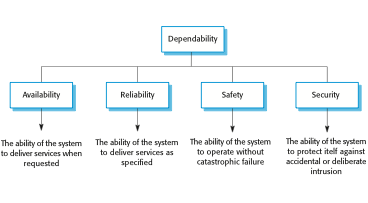
\includegraphics[width = 0.8\textwidth]{./figures/L4_1.png}
    \caption{}
    \label{fig:L4_1}
\end{figure}


\section{Principal properties}
\begin{itemize}
\item \textbf{Availability}
$-$ The probability that the system will be up and running and able to deliver useful services to users.

\item \textbf{Reliability}
$-$ The probability that the system will correctly deliver services as expected by users.

\item \textbf{Safety}
$-$ A judgment of how likely it is that the system will cause damage to people or its environment.

\item \textbf{Security}
$-$ A judgment of how likely it is that the system can resist accidental or deliberate intrusions.
\end{itemize}
 \section{Other dependability properties}
\begin{itemize}
\item \textbf{Repairability}
$-$ Reflects the extent to which the system can be repaired in the event of a failure

\item \textbf{Maintainability}
$-$ Reflects the extent to which the system can be adapted to new requirements;

\item \textbf{Survivability}
$-$ Reflects the extent to which the system can deliver services whilst under hostile attack;

\item \textbf{Error tolerance}
$-$ Reflects the extent to which user input errors can be avoided and tolerated.

\end{itemize}

\section{Repairability}
\begin{itemize}
\item The disruption caused by system failure can be minimized if the system can be repaired quickly.
\item This requires problem diagnosis, access to the failed component(s) and making changes to fix the problems.
\item Repairability is a judgment of how easy it is to repair the software to correct the faults that led to a system failure.
\item Repairability is affected by the operating environment so is hard to assess before system deployment.
\end{itemize}

\section{Maintainability}
\begin{itemize}
\item A system attribute that is concerned with the ease of repairing the system after a failure has been discovered or changing the system to include new features.
\item Repairability $-$ short-term perspective to get the system back into service; Maintainability $-$ long-term perspective.
\item Very important for critical systems as faults are often introduced into a system because of maintenance problems. If a system is maintainable, there is a lower probability that these faults will be introduced or undetected.
\end{itemize}
\section{Survivability}
\begin{itemize}
\item The ability of a system to continue to deliver its services to users in the face of deliberate or accidental attack

\item This is an increasingly important attribute for distributed systems whose security can be compromised

\item Survivability subsumes the notion of resilience - the ability of a system to continue in operation in spite of component failures

\end{itemize}
\section{Error tolerance}
\begin{itemize}
\item Part of a more general usability property and reflects the extent to which user errors are avoided, detected or tolerated.

\item User errors should, as far as possible, be detected and corrected automatically and should not be passed on to the system and cause failures.


\end{itemize}
\section{Dependability attribute examples}
\begin{itemize}
\item Safe system operation depends on the system being available and operating reliably.

\item A system may be unreliable because its data has been corrupted by an external attack.

\item Denial of service attacks on a system are intended to make it unavailable.

\item If a system is infected with a virus, you cannot be confident in its reliability or safety.

\end{itemize}
\section{Dependability achievement}
\begin{itemize}
\item Avoid the introduction of accidental errors when developing the system.

\item Design V \& V processes that are effective in discovering residual errors in the system.

\item Design protection mechanisms that guard against external attacks.

\item Configure the system correctly for its operating environment.

\item Include recovery mechanisms to help restore normal system service after a failure.

\end{itemize}
\section{Dependability costs}
\begin{itemize}
\item Dependability costs tend to increase exponentially as increasing levels of dependability are required.

\item There are two reasons for this

  \item The use of more expensive development techniques and hardware that are required to achieve the higher levels of dependability.
  \item The increased testing and system validation that is required to convince the system client and regulators that the required levels of dependability have been achieved.

\end{itemize}
\section{Cost/dependability curve}
\begin{figure}[h!]
    \centering
    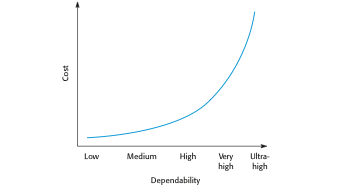
\includegraphics[width = 0.8\textwidth]{./figures/L4_2.png}
    \caption{}
    \label{fig:L4_2}
\end{figure}


\section{Dependability economics}
\begin{itemize}
\item Because of very high costs of dependability achievement, it may be more cost effective to accept untrustworthy systems and pay for failure costs

\item However, this depends on social and political factors. A reputation for products that can’t be trusted may lose future business

\item Depends on system type - for business systems in particular, modest levels of dependability may be adequate

\end{itemize}
\section{Availability and reliability}
\begin{itemize}
\item Reliability

  \item The probability of failure-free system operation over a specified time in a given environment for a given purpose

\item Availability

  \item The probability that a system, at a point in time, will be operational and able to deliver the requested services

\item Both of these attributes can be expressed quantitatively e.g. availability of 0.999 means that the system is up and running for 99.9% of the time.

\end{itemize}
\section{Availability and reliability}
\begin{itemize}
\item It is sometimes possible to subsume system availability under system reliability

  \item Obviously if a system is unavailable it is not delivering the specified system services.

\item However, it is possible to have systems with low reliability that must be available.

  \item So long as system failures can be repaired quickly and does not damage data, some system failures may not be a problem.

\item Availability is therefore best considered as a separate attribute reflecting whether or not the system can deliver its services.

\item Availability takes repair time into account, if the system has to be taken out of service to repair faults.

\end{itemize}
\section{Perceptions of reliability}
\begin{itemize}
\item The formal definition of reliability does not always reflect the user’s perception of a system’s reliability

  \item The assumptions that are made about the environment where a system will be used may be incorrect
  \newline $-$Usage of a system in an office environment is likely to be quite different from usage of the same system in a university environment
  \item The consequences of system failures affects the perception of reliability
  \newline $-$Unreliable windscreen wipers in a car may be irrelevant in a dry climate
  \newline $-$Failures that have serious consequences (such as an engine breakdown in a car) are given greater weight by users than failures that are inconvenient

\end{itemize}
\section{Reliability and specifications}
\begin{itemize}
\item Reliability can only be defined formally with respect to a system specification i.e. a failure is a deviation from a specification.

\item However, many specifications are incomplete or incorrect – hence, a system that conforms to its specification may ‘fail’ from the perspective of system users.

\item Furthermore, users don’t read specifications so don’t know how the system is supposed to behave.

\item Therefore perceived reliability is more important in practice.
\end{itemize}
\section{Availability perception}
\begin{itemize}
\item Availability is usually expressed as a percentage of the time that the system is available to deliver services e.g. 99.95%.

\item However, this does not take into account two factors:

  \item The number of users affected by the service outage. Loss of service in the middle of the night is less important for many systems than loss of service during peak usage periods.
  \item The length of the outage. The longer the outage, the more the disruption. Several short outages are less likely to be disruptive than 1 long outage. Long repair times are a particular problem.

\end{itemize}
\section{Key points}
\begin{itemize}
\item The dependability in a system reflects the user’s trust in that system.

\item Dependability is a term used to describe a set of related ‘non-functional’ system attributes – availability, reliability, safety and security.

\item The availability of a system is the probability that it will be available to deliver services when requested.

\item The reliability of a system is the probability that system services will be delivered as specified.

\end{itemize}
\section{Reliability terminology}

\begin{table}[h!]
\centering
\begin{tabular}{ |p{3cm}|p{8cm}|  }
\hline
Term & Description \\
\hline
\hline
Human error or mistake & Human behavior that results in the introduction of faults into a system. For example, in the wilderness weather system, a programmer might decide that the way to compute the time for the next transmission is to add 1 hour to the current time. This works except when the transmission time is between 23.00 and midnight (midnight is 00.00 in the 24-hour clock).\\
\hline
System fault & A characteristic of a software system that can lead to a system error. The fault is the inclusion of the code to add 1 hour to the time of the last transmission, without a check if the time is greater than or equal to 23.00.\\
\hline
System error & An erroneous system state that can lead to system behavior that is unexpected by system users. The value of transmission time is set incorrectly (to 24.XX rather than 00.XX) when the faulty code is executed.\\
\hline
System failure & An event that occurs at some point in time when the system does not deliver a service as expected by its users. No weather data is transmitted because the time is invalid.\\
\hline
\end{tabular}

\label{table:T4_1}
\end{table}

\section{Faults and failures}
\begin{itemize}
\item Failures are a usually a result of system errors that are derived from faults in the system

\item However, faults do not necessarily result in system errors

  \item The erroneous system state resulting from the fault may be transient and ‘corrected’ before an error arises.
  \item The faulty code may never be executed.

\item Errors do not necessarily lead to system failures

  \item The error can be corrected by built-in error detection and recovery
  \item The failure can be protected against by built-in protection facilities. These may, for example, protect system resources from system errors


\end{itemize}
\section{A system as an input/output mapping}
\begin{figure}[h!]
    \centering
    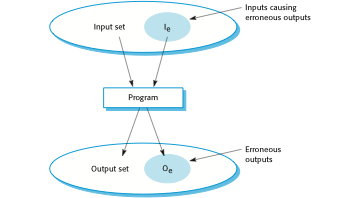
\includegraphics[width = 0.8\textwidth]{./figures/L4_3.png}
    \caption{}
    \label{fig:L4_3}
\end{figure}

\section{Software usage patterns}
\begin{figure}[h!]
    \centering
    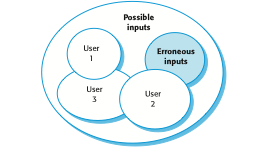
\includegraphics[width = 0.8\textwidth]{./figures/L4_4.png}
    \caption{}
    \label{fig:L4_4}
\end{figure}

\section{Reliability in use}
\begin{itemize}
\item Removing X\% of the faults in a system will not necessarily improve the reliability by X\%. A study at IBM showed that removing 60\% of product defects resulted in a 3\% improvement in reliability.

\item Program defects may be in rarely executed sections of the code so may never be encountered by users. Removing these does not affect the perceived reliability.

\item Users adapt their behaviour to avoid system features that may fail for them.

\item A program with known faults may therefore still be perceived as reliable by its users.

\end{itemize}
\section{Reliability achievement}
\begin{itemize}
\item Fault avoidance

  \item Development technique are used that either minimise the possibility of mistakes or trap mistakes before they result in the introduction of system faults.

\item Fault detection and removal

  \item Verification and validation techniques that increase the probability of detecting and correcting errors before the system goes into service are used.

\item Fault tolerance

  \item Run-time techniques are used to ensure that system faults do not result in system errors and/or that system errors do not lead to system failures.

\end{itemize}
\section{Safety}
\begin{itemize}
\item Safety is a property of a system that reflects the system’s ability to operate, normally or abnormally, without danger of causing human injury or death and without damage to the system’s environment.

\item It is important to consider software safety as most devices whose failure is critical now incorporate software -based control systems.

\item Safety requirements are often exclusive requirements i.e. they exclude undesirable situations rather than specify required system services. These generate functional safety requirements.


\end{itemize}
\section{Safety criticality}
\begin{itemize}
\item Primary safety-critical systems

  \item Embedded software systems whose failure can cause the associated hardware to fail and directly threaten people. Example is the insulin pump control system.

\item Secondary safety-critical systems

  \item Systems whose failure results in faults in other (socio-technical)systems, which can then have safety consequences. For example, the MHC-PMS is safety-critical as failure may lead to inappropriate treatment being prescribed.

\end{itemize}
\section{Safety and reliability}
\begin{itemize}
\item Safety and reliability are related but distinct

  \item In general, reliability and availability are necessary but not sufficient conditions for system safety

\item Reliability is concerned with conformance to a given specification and delivery of service

\item Safety is concerned with ensuring system cannot cause damage irrespective of whether
or not it conforms to its specification
\end{itemize}
\section{Unsafe reliable systems}
\begin{itemize}
\item There may be dormant faults in a system that are undetected for many years and only rarely arise.

\item Specification errors

  \item If the system specification is incorrect then the system can behave as specified but still cause an accident.

\item Hardware failures generating spurious inputs   \item Hard to anticipate in the specification.
\item Context-sensitive commands i.e. issuing the right command at the wrong time

  \item Often the result of operator error.
\end{itemize}
\newpage
\section{Safety terminology}
\begin{table}[h!]
\centering
\begin{tabular}{ |p{3cm}|p{8cm}|  }
\hline
Term & Definition \\
\hline
\hline
Accident (or mishap) & An unplanned event or sequence of events which results in human death or injury, damage to property, or to the environment. An overdose of insulin is an example of an accident.\\
 \hline
Hazard & A condition with the potential for causing or contributing to an accident. A failure of the sensor that measures blood glucose is an example of a hazard.\\
\hline
Damage & A measure of the loss resulting from a mishap. Damage can range from many people being killed as a result of an accident to minor injury or property damage. Damage resulting from an overdose of insulin could be serious injury or the death of the user of the insulin pump.\\
\hline
Hazard severity & An assessment of the worst possible damage that could result from a particular hazard. Hazard severity can range from catastrophic, where many people are killed, to minor, where only minor damage results. When an individual death is a possibility, a reasonable assessment of hazard severity is ‘very high’.\\
\hline
Hazard probability & The probability of the events occurring which create a hazard. Probability values tend to be arbitrary but range from ‘probable’ (say 1/100 chance of a hazard occurring) to ‘implausible’ (no conceivable situations are likely in which the hazard could occur). The probability of a sensor failure in the insulin pump that results in an overdose is probably low.\\
\hline
Risk & This is a measure of the probability that the system will cause an accident. The risk is assessed by considering the hazard probability, the hazard severity, and the probability that the hazard will lead to an accident. The risk of an insulin overdose is probably medium to low.\\
\hline
\end{tabular}

\label{table:T4_2}
\end{table}

\section{Safety achievement}
\begin{itemize}
\item Hazard avoidance

  \item The system is designed so that some classes of hazard simply cannot arise.

\item Hazard detection and removal

  \item The system is designed so that hazards are detected and removed before they result in an accident.

\item Damage limitation

  \item The system includes protection features that minimise the damage that may result from an accident.

\end{itemize}
\section{Normal accidents}
\begin{itemize}
\item Accidents in complex systems rarely have a single cause as these systems are designed to be resilient to a single point of failure

  \item Designing systems so that a single point of failure does not cause an accident is a fundamental principle of safe systems design.

\item Almost all accidents are a result of combinations of malfunctions rather than single failures.

\item It is probably the case that anticipating all problem combinations, especially, in software controlled systems is impossible so achieving complete safety is impossible. Accidents are inevitable.

\end{itemize}
\section{Software safety benefits}
\begin{itemize}
\item Although software failures can be safety-critical, the use of software control systems contributes to increased system safety

  \item Software monitoring and control allows a wider range of conditions to be monitored and controlled than is possible using electro-mechanical safety systems.
  \item Software control allows safety strategies to be adopted that reduce the amount of time people spend in hazardous environments.
  \item Software can detect and correct safety-critical operator errors.

\end{itemize}
\section{Security}
\begin{itemize}
\item The security of a system is a system property that reflects the system’s ability to protect itself from accidental or deliberate external attack.

\item Security is essential as most systems are networked so that external access to the system through the Internet is possible.

\item Security is an essential pre-requisite for availability, reliability and safety.


\end{itemize}
\section{Fundamental security}
\begin{itemize}
\item If a system is a networked system and is insecure then statements about its reliability and its safety are unreliable.

\item These statements depend on the executing system and the developed system being the same. However, intrusion can change the executing system and/or its data.

\item Therefore, the reliability and safety assurance is no longer valid.

\end{itemize}
\newpage
\section{Security terminology}
\begin{table}[h!]
\centering
\begin{tabular}{ |p{3cm}|p{8cm}|  }
\hline
Term & Definition \\
\hline
\hline
Asset & Something of value which has to be protected. The asset may be the software system itself or data used by that system.\\
\hline
Exposure & Possible loss or harm to a computing system. This can be loss or damage to data, or can be a loss of time and effort if recovery is necessary after a security breach.\\
\hline
Vulnerability & A weakness in a computer-based system that may be exploited to cause loss or harm.\\
\hline
Attack & An exploitation of a system’s vulnerability. Generally, this is from outside the system and is a deliberate attempt to cause some damage.\\
\hline
Threats & Circumstances that have potential to cause loss or harm. You can think of these as a system vulnerability that is subjected to an attack.\\
\hline
Control & A protective measure that reduces a system’s vulnerability. Encryption is an example of a control that reduces a vulnerability of a weak access control system.\\
\hline
\end{tabular}

\label{table:T4_2}
\end{table}

\section{Threat classes}
\begin{itemize}
\item Threats to the confidentiality of the system and its data

  \item Can disclose information to people or programs that do not have authorization to access that information.

\item Threats to the integrity of the system and its data   \item Can damage or corrupt the software or its data.
\item Threats to the availability of the system and its data   \item Can restrict access to the system and data for authorized users.

\end{itemize}


\section{Examples of security terminology (MHC-PMS)}
\begin{table}[h!]
\centering
\begin{tabular}{ |p{3cm}|p{8cm}|  }
\hline
Term & Example \\
\hline
\hline
Asset & The records of each patient that is receiving or has received treatment.\\
\hline
Exposure & Potential financial loss from future patients who do not seek treatment because they do not trust the clinic to maintain their data. Financial loss from legal action by the sports star. Loss of reputation.\\
\hline
Vulnerability & A weak password system which makes it easy for users to set guessable passwords. User ids that are the same as names.\\
\hline
Attack & An impersonation of an authorized user.\\
\hline
Threat & An unauthorized user will gain access to the system by guessing the credentials (login name and password) of an authorized user.\\
\hline
Control & A password checking system that disallows user passwords that are proper names or words that are normally included in a dictionary.\\
\hline
\end{tabular}

\label{table:T4_2}
\end{table}

\section{Damage from insecurity}
\begin{itemize}
\item Denial of service

  \item The system is forced into a state where normal services are unavailable or where service provision is significantly degraded

\item Corruption of programs or data

  \item The programs or data in the system may be modified in an unauthorised way

\item Disclosure of confidential information

  \item Information that is managed by the system may be exposed to people who are not authorised to read or use that information


\end{itemize}
\section{Security assurance}
\begin{itemize}
\item Vulnerability avoidance

  \item The system is designed so that vulnerabilities do not occur. For example, if there is no external network connection then external attack is impossible

\item Attack detection and elimination

  \item The system is designed so that attacks on vulnerabilities are detected and neutralised before they result in an exposure. For example, virus checkers find and remove viruses before they infect a system

\item Exposure limitation and recovery

  \item The system is designed so that the adverse consequences of a successful attack are minimised. For example, a backup policy allows damaged information to be restored
\end{itemize}
\section{Key points}
\begin{itemize}
\item Reliability is related to the probability of an error occurring in operational use. A system with known faults may be reliable.

\item Safety is a system attribute that reflects the system’s ability to operate without threatening people or the environment.

\item Security is a system attribute that reflects the system’s ability to protect itself from external attack.

\item Dependability is compromised if a system is insecure as the code or data may be corrupted.
\end{itemize}
